\newcommand{\comp}{\TT{comp()}\xspace}
\chapter{Pointers to functions}
\label{sec:pointerstofunctions}

\myindex{\CLanguageElements!\Pointers}

A pointer to a function, as any other pointer, is just the address of the function's start in its code segment.

\myindex{Callbacks}
They are often used for calling callback functions\footnote{\href{http://go.yurichev.com/17071}{wikipedia}}.

Well-known examples are:

\begin{itemize}
\item \qsort\footnote{\href{http://go.yurichev.com/17072}{wikipedia}},
{\TT{atexit()}}\footnote{\url{http://go.yurichev.com/17073}} from the standard C library; 

\item *NIX OS signals\footnote{\href{http://go.yurichev.com/17074}{wikipedia}};

\item thread starting: \TT{CreateThread()} (win32), \TT{pthread\_create()} (POSIX);

\item lots of win32 functions, like \TT{EnumChildWindows()}\footnote{\href{http://go.yurichev.com/17075}{MSDN}}.

\item lots of places in the Linux kernel, for example the filesystem driver functions are called via callbacks: 
\url{http://go.yurichev.com/17076}

\item The GCC plugin functions are also called via callbacks: 
\url{http://go.yurichev.com/17077}

\item Another example of function pointers is a table in the \q{dwm} Linux window manager that defines shortcuts.
Each shortcut has a corresponding function to call if a specific key is pressed: \href{http://go.yurichev.com/17078}{GitHub}.
As we can see, such table is easier to handle than a large switch() statement.
\end{itemize}

\myindex{\CStandardLibrary!qsort()}

So, the \qsort function is an implementation of quicksort in the \CCpp standard library. 
The functions is able to sort anything, any type of data, as long as you have a function to compare these two elements 
and \qsort is able to call it.

The comparison function can be defined as:

\begin{lstlisting}
int (*compare)(const void *, const void *)
\end{lstlisting}

Let's use a slightly modified example which was found \href{http://go.yurichev.com/17079}{here}:

\lstinputlisting[numbers=left,label=qsort_c_src]{patterns/18_pointers_to_functions/17_1.c}

\section{MSVC}

Let's compile it in MSVC 2010 (some parts were omitted for the sake of brevity) with \TT{\Ox} option:

\lstinputlisting[caption=\Optimizing MSVC 2010: /GS- /MD]{patterns/18_pointers_to_functions/17_2_msvc_Ox.asm}

Nothing surprising so far.
As a fourth argument, the address of label \TT{\_comp} is passed, which is just a place
where \comp is located, or, in other words, the address of the very first instruction of 
that function.

How does \qsort call it?

\myindex{Windows!MSVCR80.DLL}

Let's take a look at this function, located in MSVCR80.DLL (a MSVC DLL module with C standard library functions):

\lstinputlisting[caption=MSVCR80.DLL]{patterns/18_pointers_to_functions/17_3_MSVCR.lst}

\TT{comp}---is the fourth function argument.
Here the control gets passed to the address in the \TT{comp} argument.
Before it, two arguments are prepared for \comp. Its result is checked after its execution.

That's why it is dangerous to use pointers to functions.
First of all, if you call \qsort with an incorrect function pointer, \qsort may pass control flow
to an incorrect point, the process may crash and this bug will be hard to find.

The second reason is that the callback function types must comply strictly, calling the wrong function
with wrong arguments of wrong types may lead to serious problems, however, the crashing of the process is not a 
problem here~---the problem is how to determine the reason for the crash~---because the compiler may be 
silent about the potential problems while compiling.

\clearpage
\subsectionold{MSVC + \olly}
\myindex{\olly}

Let's load our example into \olly and set a breakpoint on \comp.
We can see how the values are compared at the first \comp call:

\begin{figure}[H]
\centering
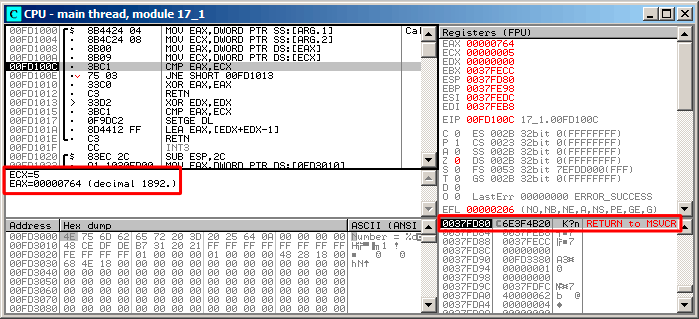
\includegraphics[scale=\FigScale]{patterns/18_pointers_to_functions/olly1.png}
\caption{\olly: first call of \comp}
\label{fig:qsort_olly1}
\end{figure}

\olly shows the compared values in the window under the code window, for convenience.
We can also see that the \ac{SP} points to \ac{RA}, where the \qsort function is (located in \TT{MSVCR100.DLL}).

\clearpage
By tracing (F8) until the \TT{RETN} instruction and pressing F8 one more time, we return to the \qsort function:

\begin{figure}[H]
\centering
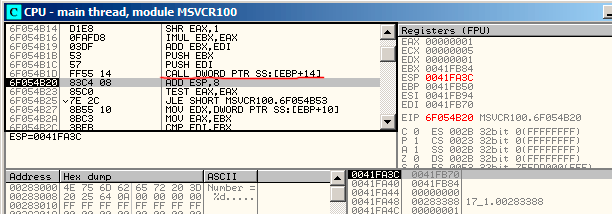
\includegraphics[scale=\FigScale]{patterns/18_pointers_to_functions/olly2.png}
\caption{\olly: the code in \qsort right after \comp call}
\label{fig:qsort_olly2}
\end{figure}

That was a call to the comparison function.

\clearpage
Here is also a screenshot of the moment of the second call of \comp{}---now values that have to be compared are different:

\begin{figure}[H]
\centering
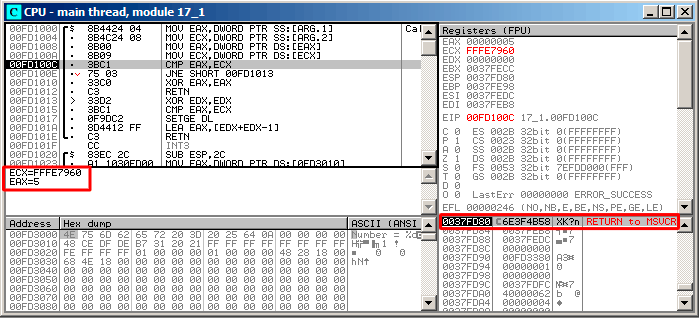
\includegraphics[scale=\FigScale]{patterns/18_pointers_to_functions/olly3.png}
\caption{\olly: second call of \comp}
\label{fig:qsort_olly3}
\end{figure}


\subsection{MSVC + tracer}
\myindex{tracer}

Let's also see which pairs are compared.
These 10 numbers are being sorted: 
1892, 45, 200, -98, 4087, 5, -12345, 1087, 88, -100000.

We got the address of the first \CMP instruction in \comp, it is \TT{0x0040100C} and we've set a breakpoint on it:

\begin{lstlisting}
tracer.exe -l:17_1.exe bpx=17_1.exe!0x0040100C
\end{lstlisting}

Now we get some information about the registers at the breakpoint:

\begin{lstlisting}
PID=4336|New process 17_1.exe
(0) 17_1.exe!0x40100c
EAX=0x00000764 EBX=0x0051f7c8 ECX=0x00000005 EDX=0x00000000
ESI=0x0051f7d8 EDI=0x0051f7b4 EBP=0x0051f794 ESP=0x0051f67c
EIP=0x0028100c
FLAGS=IF
(0) 17_1.exe!0x40100c
EAX=0x00000005 EBX=0x0051f7c8 ECX=0xfffe7960 EDX=0x00000000
ESI=0x0051f7d8 EDI=0x0051f7b4 EBP=0x0051f794 ESP=0x0051f67c
EIP=0x0028100c
FLAGS=PF ZF IF
(0) 17_1.exe!0x40100c
EAX=0x00000764 EBX=0x0051f7c8 ECX=0x00000005 EDX=0x00000000
ESI=0x0051f7d8 EDI=0x0051f7b4 EBP=0x0051f794 ESP=0x0051f67c
EIP=0x0028100c
FLAGS=CF PF ZF IF
...
\end{lstlisting}

Let's filter out \TT{EAX} and \TT{ECX} and we got:

\begin{lstlisting}
EAX=0x00000764 ECX=0x00000005
EAX=0x00000005 ECX=0xfffe7960
EAX=0x00000764 ECX=0x00000005
EAX=0x0000002d ECX=0x00000005
EAX=0x00000058 ECX=0x00000005
EAX=0x0000043f ECX=0x00000005
EAX=0xffffcfc7 ECX=0x00000005
EAX=0x000000c8 ECX=0x00000005
EAX=0xffffff9e ECX=0x00000005
EAX=0x00000ff7 ECX=0x00000005
EAX=0x00000ff7 ECX=0x00000005
EAX=0xffffff9e ECX=0x00000005
EAX=0xffffff9e ECX=0x00000005
EAX=0xffffcfc7 ECX=0xfffe7960
EAX=0x00000005 ECX=0xffffcfc7
EAX=0xffffff9e ECX=0x00000005
EAX=0xffffcfc7 ECX=0xfffe7960
EAX=0xffffff9e ECX=0xffffcfc7
EAX=0xffffcfc7 ECX=0xfffe7960
EAX=0x000000c8 ECX=0x00000ff7
EAX=0x0000002d ECX=0x00000ff7
EAX=0x0000043f ECX=0x00000ff7
EAX=0x00000058 ECX=0x00000ff7
EAX=0x00000764 ECX=0x00000ff7
EAX=0x000000c8 ECX=0x00000764
EAX=0x0000002d ECX=0x00000764
EAX=0x0000043f ECX=0x00000764
EAX=0x00000058 ECX=0x00000764
EAX=0x000000c8 ECX=0x00000058
EAX=0x0000002d ECX=0x000000c8
EAX=0x0000043f ECX=0x000000c8
EAX=0x000000c8 ECX=0x00000058
EAX=0x0000002d ECX=0x000000c8
EAX=0x0000002d ECX=0x00000058
\end{lstlisting}

That's 34 pairs.
Therefore, the quick sort algorithm needs 34 comparison operations to sort these 10 numbers.

\clearpage
\subsection{MSVC + tracer (code coverage)}
\myindex{tracer}

We can also use the tracer's feature to collect all possible register values and show them in \IDA.

Let's trace all instructions in \comp:

\begin{lstlisting}
tracer.exe -l:17_1.exe bpf=17_1.exe!0x00401000,trace:cc
\end{lstlisting}

We get an .idc-script for loading into \IDA and load it:

\begin{figure}[H]
\centering
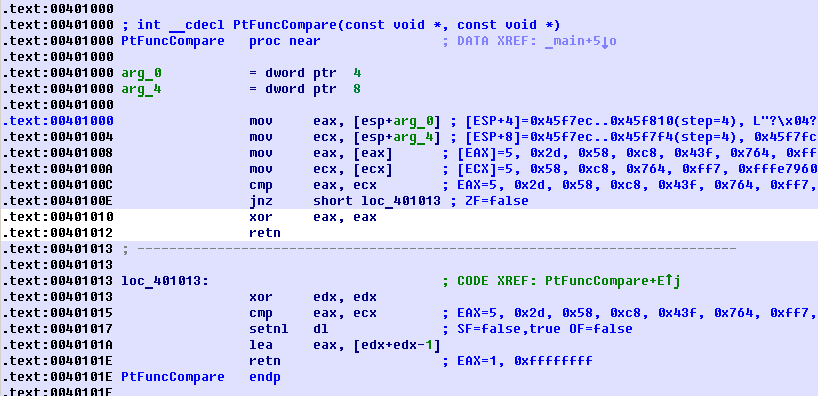
\includegraphics[scale=\FigScale]{patterns/18_pointers_to_functions/tracer_cc.png}
\caption{tracer and IDA. N.B.: 
some values are cut at right}
\label{fig:qsort_tracer_cc}
\end{figure}

\IDA gave the function a name (PtFuncCompare)---because \IDA sees that the pointer to this function is passed to \qsort.

We see that the $a$ and $b$ pointers are pointing to various places in the array, but the step between
them is 4, as 32-bit values are stored in the array.

We see that the instructions at \TT{0x401010} and \TT{0x401012} were never executed (so they left as white): 
indeed, \comp has never returned 0, because there no equal elements in the array.

\section{GCC}

Not a big difference:

\begin{lstlisting}[caption=GCC]
                lea     eax, [esp+40h+var_28]
                mov     [esp+40h+var_40], eax
                mov     [esp+40h+var_28], 764h
                mov     [esp+40h+var_24], 2Dh
                mov     [esp+40h+var_20], 0C8h
                mov     [esp+40h+var_1C], 0FFFFFF9Eh
                mov     [esp+40h+var_18], 0FF7h
                mov     [esp+40h+var_14], 5
                mov     [esp+40h+var_10], 0FFFFCFC7h
                mov     [esp+40h+var_C], 43Fh
                mov     [esp+40h+var_8], 58h
                mov     [esp+40h+var_4], 0FFFE7960h
                mov     [esp+40h+var_34], offset comp
                mov     [esp+40h+var_38], 4
                mov     [esp+40h+var_3C], 0Ah
                call    _qsort
\end{lstlisting}

\comp function:

\begin{lstlisting}
                public comp
comp            proc near

arg_0           = dword ptr  8
arg_4           = dword ptr  0Ch

                push    ebp
                mov     ebp, esp
                mov     eax, [ebp+arg_4]
                mov     ecx, [ebp+arg_0]
                mov     edx, [eax]
                xor     eax, eax
                cmp     [ecx], edx
                jnz     short loc_8048458
                pop     ebp
                retn
loc_8048458:
                setnl   al
                movzx   eax, al
                lea     eax, [eax+eax-1]
                pop     ebp
                retn
comp            endp
\end{lstlisting}

\myindex{Linux!libc.so.6}

The implementation of \qsort is located in \TT{libc.so.6} and it is in fact just a wrapper
\footnote{a concept like \gls{thunk function}} for \TT{qsort\_r()}.

In turn, it is calling \TT{quicksort()}, where our defined function is called via a passed pointer:

\begin{lstlisting}[caption=(file libc.so.6{,} glibc version---2.10.1)]

.text:0002DDF6                 mov     edx, [ebp+arg_10]
.text:0002DDF9                 mov     [esp+4], esi
.text:0002DDFD                 mov     [esp], edi
.text:0002DE00                 mov     [esp+8], edx
.text:0002DE04                 call    [ebp+arg_C]
...
\end{lstlisting}

\subsection{GCC + GDB (with source code)}
\myindex{GDB}

Obviously, we have the C-source code of our example (\myref{qsort_c_src}), 
so we can set a breakpoint ($b$) on line number (11---the line where the first comparison occurs).
We also need to compile the example with debugging information included (\TT{-g}), so the table
with addresses and corresponding line numbers is present.

We can also print values using variable names (\TT{p}):
the debugging information also has tells us which register and/or 
local stack element contains which variable.

\myindex{Glibc}
We can also see the stack (\TT{bt}) and find out that there is some intermediate function \TT{msort\_with\_tmp()} used in Glibc.

\lstinputlisting[caption=GDB session]{patterns/18_pointers_to_functions/GDB_source.txt}

\subsection{GCC + GDB (no source code)}
\myindex{GDB}

But often there is no source code at all, so we can disassemble the \comp function (\TT{disas}), find the very first
\CMP instruction and set a breakpoint ($b$) at that address.

At each breakpoint, we are going to dump all register contents (\TT{info registers}).
The stack information is also available (\TT{bt}), 

but partially: there is no line number information for \comp.

\lstinputlisting[caption=GDB session]{patterns/18_pointers_to_functions/GDB_no_source.txt}

